%\documentclass[twoside,a4paper]{report}
\documentclass[a4paper, twocolumn]{article}

\usepackage[utf8]{inputenc}

\usepackage{hyperref}
\usepackage{graphicx}
\usepackage{tabularx}
\usepackage{booktabs}
\usepackage{supertabular}
\usepackage{multirow}
\usepackage{varwidth}

\newcommand{\turn}[3][10em]{% \turn[<width>]{<angle>}{<stuff>}
  \rlap{\rotatebox{#2}{\begin{varwidth}[t]{#1}\bfseries#3\end{varwidth}}}%
  }

\usepackage{pdflscape} %% Used for very big table
\usepackage{moreverb}
\usepackage[table]{xcolor}
\usepackage{listings}
\usepackage{paralist}
\usepackage{fancyhdr}
\usepackage[draft]{fixme}
\fxsetup{footnote}
\fxsetup{nomargin}

\definecolor{codegray}{gray}{.95}
\definecolor{palegray}{gray}{.65}
\lstset{language=C,
	numbers=left,
	tabsize=2,
	basicstyle=\scriptsize,
	stringstyle=\textrm,
	showstringspaces=false,
	frame=none,
	xleftmargin=3pt,
	backgroundcolor=\color{codegray}}

\title{Requirements and Current State of Knowledge Representation Systems for Service Robotics}
\author{Séverin Lemaignan, Moritz Tenorth, Michael Beetz}

\graphicspath{{figs/}}

\newcommand{\concept}[1]{{\footnotesize \texttt{#1}}}
\newcommand{\ie}{{\textit{i.e.~}}}
\newcommand{\cf}{{\textit{cf~}}}
\newcommand{\eg}{{\textit{e.g.~}}}

\newcommand{\stmt}[1]{{\footnotesize \tt $\langle$ #1\relax$\rangle$}}
%\newcommand{\stmt}[1]{{\footnotesize $\langle$\stmttt#1\relax$\rangle$}}
\newcommand{\rawstmt}[1]{{\footnotesize \stmttt#1\relax}}
\def\stmttt#1 #2 #3\relax{{\tt#1} {\bf{\tt #2}} {\tt #3}}

\newcommand{\setstmt}[1]{{\footnotesize [\setstmttt#1\relax]}}
\def\setstmttt#1,#2\relax{\rawstmt{#1}, \rawstmt{#2}}


\begin{document}

\maketitle
\tableofcontents


\begin{abstract}

The aim of this contribution is two-fold: we first propose a typology of
knowledge representation systems for service robotics that covers intrinsic
features like expressiveness or reasoning techniques as well as extrinsic
features like knowledge acquisition and integration into pre-existent robotic
architectures.

We then survey the current knowledge representation system in the community to
identify which knowledge-bound cognitive abilities are today well understood
and implemented, and which would require more efforts.

We hope this article may bring a clearer picture of the challenges of knowledge
representation and manipulation for the robotics research community.

\end{abstract}

%%%%%%%%%%%%%%%%%%%%%%%%%%%%%%%%%%%%%%%%%%%%%%%%%%%%%%%%%%%%%%%%%%%%%%%%%%%%%%%%%%%%%%%%%%%
\section{Introduction}
\label{sect|intro}

\subsection{Knowledge as the Root of Cognitive Abilities}
\label{sect|cognitive-abilities}

The idea of \emph{Cognitive Robotics} was coined in the early 1990s by Reiter.
In a chapter on that subject in \emph{Fondations of Artifical
Intelligence}~\cite{Levesque2008}, Levesque reminds about the manifesto they
wrote together in 1998:

\begin{quotation}

    Central to this effort is to develop an understanding of the relationship
    between the knowledge, the perception, and the action of \[...\] a robot. The
    sorts of questions we want to be able to answer are

    \begin{itemize} 

        \item to execute a program, what information does a robot need to have
        at the outset vs. the information that it can acquire \emph{en route}
        by perceptual means?

        \item what does the robot need to know about its environment vs. what
        need only be known by the designer?

        \item when should a robot use perception to find out if something is
        true as opposed to reasoning about what it knows was true in the past?

        \item when should the inner workings of an action be available to the
        robot for reasoning and when should the action be considered primitive
        or atomic?

    \end{itemize}

    and so on. With respect to robotics, our goal (like that of many in AI) is
    \emph{high-level robotic control}: develop a system that is capable of
    generating actions in the world that are appropriate as a function of some
    current set of beliefs and desires.

\end{quotation}

Those questions have in common one prerequisite to be answered: the robot must
be able to manipulate \emph{explicitely} knowledge, and hence, need a wayto
represent the knowledge.

This survey focuses on this knowledge representation issue: we aims at first
establishing a as-exhaustive-as-possible typology of representation needs for
robotics, and then at painting the current landscape of approaches to the
knowledge representation problem in the research community, in order to
summarize the major trends and to identify the possible shortcomings.

We have classified the features of knowledge representation systems (KRS) into
six broad categories: \emph{what can be represented?} or the
\emph{expresiveness} question ; \emph{how things are represented?} ; \emph{what
reasoning techniques are offered?} ; \emph{how knowledge is acquired and
anchored?} ; \emph{how the knowledge is made available and used by the other
components of the robot?} and \emph{which actual knowledge is stored?} or the
\emph{knowledge instanciation} question.

We have identified over ten projects that are either explicitely advertised as
knowledge representation systems or involve explicit knowledge manipulation
within a robot. By knowledge manipulation, we mean symbolic representation of
assertions, be it static statements on the world or spatio-temporal events, and
reasoning on this representation. Proeminent features of each of these systems
illustrate how the various features of a knowledge representation system are
currently implemented.

We have also tried, for each project, to make clear \begin{inparaenum} \item
how informations from perception or interaction are turned into knowledge,
\item how, in return, symbolic concept are \emph{anchored} into the robot
sensori-motor space, \item how the knowledge representation system integrates
with the decisional layers of the robot, and how this can improve or ease
robotic control.\end{inparaenum}

\subsection*{A Note on Terminology}

Since this article discusses at length the concept of knowledge in the context
of robotics, it is useful to make our terminology explicit.  No general
agreement on a definition of ``knowledge'' exists. In our context, we call
``knowledge'' \emph{an explicit set of interrelated logical facts that are
meaningful to the robot executive controller} (by \emph{meaningful} we mean
that can possibly be interpreted to lead to a purposeful action).

The relation of \emph{data} and \emph{information} to knowledge is a debated
epistemology question (the interested reader is invited to refer to the
Wikipedia page on the ``DIKW'' hierarchy). In this article, we will associate
data to low-level material like raw sensor output, and information to
uncontextualized symbolic facts.

To give a example, image a human watching at a book and being tracked by a
Kinect sensor: the pose of the human skeleton in the world would be the data,
the fact \concept{looksAt(human, book)} as computed by a geometric reasoning
module would be the information, the fact \concept{looksAt(john,
war\_and\_peace)}, fully grounded and connected to the whole knowledge base of
the robot would be proper knowledge.

\subsection*{Survey Inclusion Criteria}
\label{sect|inclusion-criteria}

Every robotic system has, implicitely or not, some knowledge representation
systems. It may range from a simple state vector to an explicit symbolic
knowledge base.  This survey focuses on the right end of this spectrum:
symbolic systems, suited for abstract reasoning.

Besides, we have decided to restraint the set of systems to those actually
implemented on robots, and used in semantic-rich environments (\ie , dynamic,
partially unknown environments with a large range of different entities which
may have interactions). The typical scenario that would involve such robots is
a service robot in a human-friendly environment like a kitchen (as described in
section~\ref{sect|scenario}).

We have limited ourselves to systems that
\begin{inparaenum} 
    \item  run on \emph{service robot} (that is, robots that interact with 
    objects in a semantic-rich environment primarly designed for humans),
    \item  ground the knowledge in the physical world (physically embedded
    systems able to assess their environment),
    \item  are able to merge different knowledge modalities,
    \item  are able of on-line, dynamic knowledge acquisition and reasoning 
    (\ie not a simple static database).
\end{inparaenum}

While classical cognitive systems like {\sc Soar} or {\sc ACT-R} have
declarative knowledge modules and have been recently used on service robots
(see {\sc ACT-R/E}~\cite{Kennedy2009} for instance), they are absent from this
survey because we could not find evidence in the litterature on possible
on-line manipulation of symbolic knowledge.

\subsection{Previous Work}
\label{sect|evaluation-literature}

To the extend of our knowledge, no previous published work attempt to build a
typology of cognitive abilities related to knowledge and required by service
robotics.

However, several authors from fields that are connected to the robotics have
previously listed desirable features of artificial systems aiming at cognitive
abilities as rich as possible.

For instance, in~\cite{McCarthy2007}, McCarthy recently listed the challenges
he identifies on the road to a \emph{human-level AI}.

\begin{itemize}

	\item the ability to \emph{"operate successfully in the common sense
	informatic situation"},

	\item the necessity of relying on mathematical logic, as the most fruitful
	formalism for machine intelligence,

	\item the ability to deal with \emph{approximate concepts and approximate
	theories} (that would include representing them, and reasoning with them),

	\item non-monotonic reasoning,

	\item what McCarthy calls \emph{Elaboration Tolerance}: the ability to
	extend \emph{on demand} the closed domain of interpretation for a
	given assertion,

	\item the ability to formalize and reason about contexts,

	\item reasoning about events, and in particular, actions,

	\item the capacity of introspection,

	\item and finally, he points the issue of giving computer the right
	heuristics for decision making.

\end{itemize}

Several surveys compare global cognitive architectures (\cite{Vernon2007, Chong2009}).
Vernon et al.~\cite{Vernon2007} split these architectures into two broad
categories: the \emph{cognitivist} ones (where cognition is considered as an
explicit computation problem, often based on symbol manipulation), and the
\emph{emergent} ones (where cognition only exists as a result of the
interaction of the system with its environment). The approaches presented in
this paper are, at a few exceptions, prototypical \emph{cognitivist} approaches
that aim at making knowledge explicit within the robot architecture. Vernon et
al. propose twelve \emph{characteristics of cognitive system} to compare
architectures. Amongst them, they mention the \emph{inter-agent epistemology} (how
the structure of the world is captured in a representation and shared), the
relation to \emph{embodiement}, the ability to \emph{anticipate} and to
\emph{adapt}, and the mechanisms of \emph{motivation}. While presented at the
level of the whole robotic architecture, these features also translate into
knowledge representation strategies and are relevant to our study.

Coming from the perspective of natural language processing in situated context,
Roy and Reiter, in~\cite{Roy2005}, summarize what they see as the main
challenges to be tackled by KRS: cross-modal representation systems, association of
words with perceptual and action categories, modeling of context, figuring out
the right granularity of models, integrating temporal modeling and planning,
ability to match past (learned) experiences with the current interaction and
ability to take into account the human perspective.

Knowledge representation systems in robotics are concerned by most, if not all,
of these points, and we shall reuse them later, in slightly reformulated ways.

\subsection{Article overview}
\label{sect|overview}

The paper is organized in four main sections.

The next section proposes a prototypical scenario in a rich semantic
environment. We will not survey knowledge representation systems based on this
scenario: we merely use it to ground the selection and illustrate the set
features that define the dimensions of a
knowledge representation system for robotics.

Section~\ref{sect|features} presents these features in detail, and organize
them into a typology.

Section~\ref{sect|surveyed-systems} then presents each of the systems we
examinated, and underlines their specificities.

We finally summarize in section~\ref{sect|summary} the current approaches in
relation to the previously identified set of features. This leads us to
identify several new research directions that are not sufficiently addressed by
the current state of the art.

%%%%%%%%%%%%%%%%%%%%%%%%%%%%%%%%%%%%%%%%%%%%%%%%%%%%%%%%%%%%%%%%%%%%%%%%%%%%%%%%%%%%%%%%%%%
\section{A Prototypical Scenario}
\label{sect|scenario}

\begin{figure*}
	\centering
	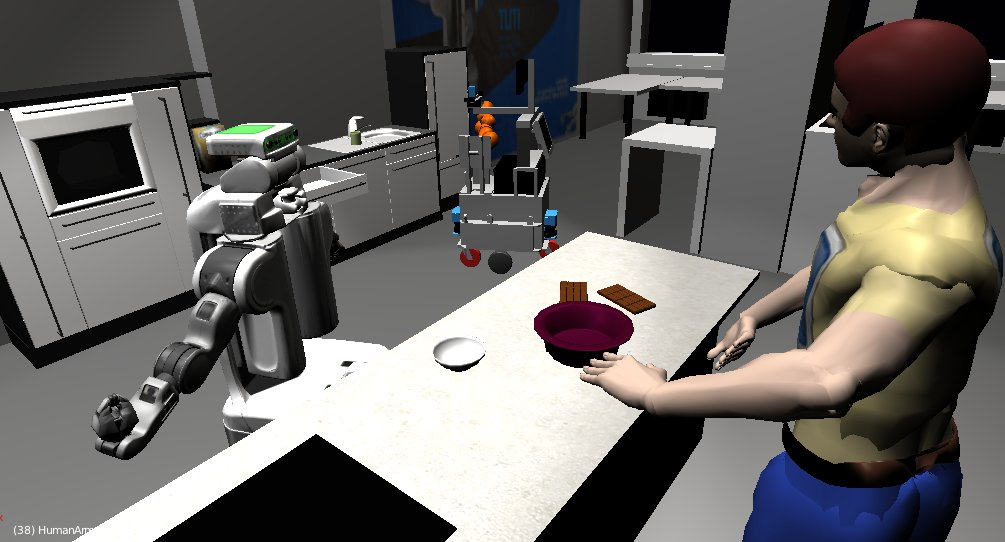
\includegraphics[width=0.9\textwidth]{figs/brownie_scenario.jpg}
	\caption{A possible representation of the scenario, in the MORSE simulator}
	\label{fig|scenario}
\end{figure*}

In order to illustrate what we consider to be the required features of a
knowledge representation system for robotics, we introduce in this section a
demonstration scenario.

While devising a scenario inevitably constraints the breadth of abilities we
examine, we insist on the fact that our main purpose here is to ground into a
real case the set of representational features we consider as desirable.  We
will \emph{not} evaluate any of the systems we survey in this article by
judging their applicability to this particular scenario.

We entitle our scenario ``the Brownie scenario'' (Fig.~\ref{fig|scenario}).

Robi and Roba are two service robots. They are considered to be able to freely
move and pick objects, but they are not expected to have the exact same
hardware and softwares architectures, and specially, they are not expected to
have the same knowledge representation system. These robots cooperate with a
human in a kitchen environment.

The main task of the scenario is the joint realization of a brownie, initiated
by the human injunction ``Let's make a brownie for tonight!''.

The scenario is successful if the task is achieved (the brownie is baked) and:

\begin{itemize} 

	\item it took less time that it would have require for the human alone, 

	\item it didn't require a heavier cognitive involvement from the human that
	what would have been required without the robots' help.  

\end{itemize}

We voluntarily do not detail the subtasks of the scenario, neither we define
how they are shared amongst agents. In our analysis we focus on the general,
\textit{a priori} representational needs of the scenario.

A ``first-order'' analysis of this task leads to a rough partition of the
required representation abilities:

\begin{enumerate}

	\item Representation abilities related to the execution of a complex
	spatio-temporal task,

	\item Representation abilities related to cooperation with other agents.

\end{enumerate}

% Representation of a complex task
We can further refine these categories: to prepare and bake a brownie, the
robot first needs to make sense of the very term \emph{brownie}: what is it?
what is it used for? what is it made of? etc. We call this knowledge
\emph{common-sense knowledge} and the robot must be able not only to represent
it, but also to have some kind of access to it (for instance through a initial
set of facts that are made available at startup, or via access to a Web-based
knowledge base like Wikipedia, etc.)

Bound to the action \emph{make}, this should lead the robot to build and
represent a \emph{context}: we are in a scenario involving cooking. Actions
related to cooking often take place in the kitchen, cooking requires ingredients, 
utensils and a procedure that may be provided by a recipe, etc.

This last sentence implies several other features for our knowledge
representation system: ``cooking often takes place in the kitchen'' implies
that representation of both uncertainty and likelihood is desirable. The fact
that cooking is associated to a place further implies that the system models
locations and is able to attach \emph{thematic relations} to concept
(here, the likely location of the cooking action).

``cooking requires ingredients that may be provided by a recipe'' hints about a
very common feature available in most knowledge representation systems:
\emph{reasoning}. The robot \emph{infers} that cooking may require a recipe
since a list of ingredients is a pre-requisite of the cooking action, and a
recipe may provide such a list. If we omit the ``may'', this is a typical
example of first-order logic reasoning. Many other reasoning techniques exist
(including probabilistic ones -- ones able to deal with the ``may''), we shall
illustrate some of them later in this scenario.

We mentioned that a recipe often provides a procedure (or a \emph{plan}). The
robot should be able to store this plan in a way that allow later execution.
The plan is likely to contain \emph{spatio-temporal constraints} (like ``put
the brownie in the oven for 20 min'' or ``let's cook \emph{for tonight}'') that
must as well be appropriately represented.

To make decision, a robot may also want to \emph{predict} the state of the world
after some action (``if I leave the cake 2h in the oven, it will burn'').
Such ability to project itself in future or, generally speaking, in other
possible state of the world is related to several cognitive ability and
reasoning techniques: \emph{planning}, \emph{representation of possible worlds}
and \emph{non-monotonic reasoning}, in addition to common-sense knowledge and
\emph{physics-based} reasoning (that allows to predict that an egg is likely to
break if dropped).

Procedures are in addition often \emph{underspecified}: we can expect the recipe
to provide a cooking duration, but we usually do not expect the recipe to tell
us to first open the oven door, and then put the cake into it, since it is
self-evident that the door must first be opened to put the cake in the oven.
Such underspecification should be detectable, representable, and ideally
completable by the knowledge representation system\footnote{Note that we do not
assume here the {\it knowledge representation system} to be a single software
component: it may well be the result of the aggregation of several logical
components working together}.

% Representation feature that enable cooperation
Then, we want our three agents to cooperate. This, in turn, leads to another
set of cognitive abilities.

Cooperation in our scenario can intervene at many places. For instance, an
agent may want to inform another one about the number of eggs that are
necessary for the brownie. This \emph{helping} behaviour makes sense only if
the first agent knows that the recipient agent both needs the information but
does not know it. This in turn requires the robot to be able to model the
knowledge of the other agents: to think \emph{from the perspective} of another
agent (this idea is related to the so-called Theory of Mind~\cite{Leslie2000}).

Ability to communicate is one important pre-requisite to collaboration.
Communication in general~\cite{Jakobson1960} requires the addresser and the
addressee to share a common interpretative framework (a shared common-sense
knowledge -- or cultural background -- and a shared context). In our scenario,
the agents are working in a kitchen. This element of context does not however
suffice if, for example, an agent asks another agent to ``give {[him]} the
bowl''. Behind the symbol ``bowl'', which physical entity are we actually
talking about? If we want to act on the world, this so-called \emph{grounding}
operation is essential, and may be tightly bound to the underlying knowledge
representation system. Note that grounding usually denotes the {\it top-down}
operation: from the symbol to the percept. It is however commonly bundled with
the converse operation, that retrieve (or create) symbols from perception.

A related ability is called \emph{pre-supposition accomodation}: if one of the
agent moves behind another one, with the brownie dough in its arm, and says
``be careful, I'm behind you!'', we want the first agent to be able to
represent both symbolically and geometrically (because, for instance, if the
agent want to move, it must take into account the new obstacle) something that
was not directly perceived. A knowledge representation system may be able to
provide structures to represent and reason about such cases.

Also central to cooperation are the notions of \emph{joint
intentions} and \emph{joint goals}~\cite{Tomasello2005, Bratman2009}: to help
the human during the cooking session, the robots need to track how far
they are into the recipe, what is the next step the human is likely to go for,
how task are currently split between agents, what action is currently
blocking the procedure, etc. This knowledge should let the robot identify the
intentions of other agents and create accordingly joint goals. Hence, a
knowledge representation system aiming at dealing with cooperative behaviours
is likely to have goal management structures taking explicitly into account
other agents' actions and goals.

In order to effectively share tasks, the robot must also know what it is
capable of: \emph{capability introspection} (both in term of general capability
and of immediate ability) is thus often desirable. More general introspection
(like the ability to tell ``who I am'' or ``what do I think of'' does not
appear to be necessary in our scenario. This may however be required in more
general human-robot interaction.

Last but not least, our scenario assumes implicitly \emph{natural interaction}
between humans and robots (as showed by the casual style of the
order ``Let's make a brownie!''). While natural language processing {\it
per-se} is usually out of the scope of a knowledge representation system, we
may want to be sure these systems may successfully interoperate, \ie that the
knowledge representation system provides efficient support to the natural
language processing module (for instance by adopting models and vocabulary that
are both well suited for machine processing and remain as close as possible to
the humans own structures and vocabulary).

%%%%%%%%%%%%%%%%%%%%%%%%%%%%%%%%%%%%%%%%%%%%%%%%%%%%%%%%%%%%%%%%%%%%%%%%%%%%%%%%%%%%%%%%%%%
\section{A Typology of Knowledge Representation Systems Requirements for Robotics}
\label{sect|features}

We presented an imaginary cooking scenario where numerous desirable
features for a knowledge representation system for robotics have been
identified in no particular order.

This section proposes a more formal typology of desirable features for a such a
system. For each feature, we provide a short definition along with links to
relevant literature.

Table~\ref{table|contribution-by-systems}, at the end of the article,
summarizes all these features with the main domain of contribution of each
surveyed KRS.

\subsection{Expressiveness: What Can be Represented?}
\label{sect|expressiveness}

\subsubsection{Introduction: Main Logic Formalisms}

The main role of a knowledge representation system is to provide an adequate
representation system to store facts and concepts that can be informally
described in natural language.

Formal logic aims at providing such a representation system with the added
value of providing a tractable support for inference and reasoning.

Most (but not all) of the systems we survey rely on a particular logic
formalism. The choice of the formalism has a strong impact, on one side, on the
range of ideas that can be expressed conveniently (\emph{practical
expressiveness}) or at all (\emph{theoretical expressiveness}), on the other
side, on the ability to solve the inference problem (called
\emph{satisfiability}: is a given logical sentence true in my model?) in a
tractable manner.

A large number of logic formalism do exist, we shall summarize below the most
relevant for systems actually deployed in current robotic architectures.

\emph{Predicate logic} is the family of logic formalisms the most commonly
found in knowledge representation. It distinguishes itself from the simpler
\emph{propositional logic} by the use of quantification to increase generality.
\emph{First-order logic} (FOL) is the subpart of \emph{predicate logic} where the
objects of \emph{predicates} (or \emph{formulae}) are simple \emph{terms},
while in \emph{higher-order logics}, predicates can be themselves objects of
other predicates.

\emph{Horn clauses} are an important subset of FOL because the satisfiability
of a set of such clauses is a $P$-complete problem. A Horn clause is a
disjunction of literals (a \emph{clause}) with at most one positive literal:
$\neg p \vee \neg q \vee \cdots \vee \neg t \vee u$, which can also be
represented as $(p \wedge q \wedge \cdots \wedge t) \rightarrow u$.  Important
logic programming languages like Prolog are based on Horn clauses.

The family of \emph{Description Logics}~\cite{Baader2008} also play an
important role. It is also a subset of the first-order logic, with some
extensions in second-order logic. Description logics are notable because most
of them are known to be decidable. In description logic, axioms are build from
\emph{concepts}, \emph{roles} (that are unary or binary predicates) and
\emph{individuals}. The W3C OWL-DL standard is a widely-used language to
describe domains with the description logic.

Because Description Logics have been originally created from the perspective of
a \emph{knowledge representation language} and not a logic language, their
terminology (\emph{concept} or \emph{class}, \emph{role} or \emph{property},
\emph{individual},...) is well-suited to knowledge description and we may use
it in the remaining of this paper outside of the strict context of  Description
Logics.

\emph{Modal logic}, that allow for statement qualification like
\emph{possibility} or \emph{necessity}, have been shown to be closely related
to description logics. Modal logic allows to represent conveniently parallel
possible worlds and facts like ``the robot knows \emph{that the human knows}
how to read a recipe''.

\fxfatal{On modal logics, see the remark of McCarthy, in \cite{McCarthy2007}, section 3}

\emph{Temporal logic} are designed to represent and manipulate assertions whose
truth value may vary in time.

One last class of logics that is of particular relevance for robotic
applications is the \emph{probabilistic logics} or \emph{Bayesian logics}.
These logics provide a formal framework to reason on propositions whose truth
or falsity is uncertain. We elaborate below on the representation of uncertainty.

Note that most of these logic formalisms are still active research field by
their own, and practical considerations (especially the availability of
reasoners performant enough for on-line use on a robot) often constraint the
choice of a logical formalism and a level of expressive power.


\paragraph{Some examples}

\emph{The robot knows that a blue bottle is laying on the table.}

\emph{The robot knows that the human knows about the position of the bottle,
but the robot does not know what the human actually know about it.}

\subsubsection{Expressive Power}

Logical formalisms each bring a certain level of expressive power. For
instance, the following classical syllogism can not be represented in
propositional logic because of the use of \emph{universal quantification}:

\begin{quote}
\begin{enumerate}
    \item All men are mortal,
    \item Socrates is a man,
    \item Therefore, Socrates is mortal
\end{enumerate}
\end{quote}

However, the following weak version of the syllogism can be represented in
propositional logic:

\begin{quote}
\begin{enumerate}
    \item If Socrates is a man, then Socrates is mortal,
    \item Socrates is a man,
    \item Therefore, Socrates is mortal
\end{enumerate}
\end{quote}

Generally speaking, expressive power comes at the cost of more complex
\emph{satisfiability} and \emph{consistency}\footnote{We precise these concepts
at section~\ref{sect|reasoning}.} computations, possibly leading to
untractable, if not undecidable (\ie systems where it is proven that a
proposition can not be decided to be true or false) problems.

\begin{figure}
    \centering
    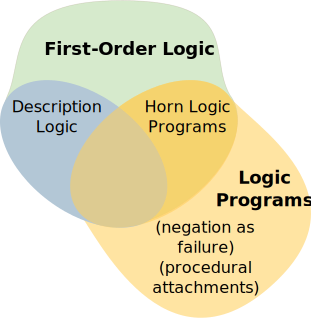
\includegraphics[width=0.6\columnwidth]{expressive_overlap_dl_horn.pdf}
    \caption{Expresiveness overlap of Description Logics and logic programs
    based on Horn clauses, taken from~\cite{Grosof2003}}
    \label{fig|overlap_dl_horn}
\end{figure}

Figure~\ref{fig|overlap_dl_horn} shows that the expresive power of description
logics and Horn clauses partially overlaps. In section~\ref{sect|reasoning} we
mention extensions to description logics based on rule systems to bring closer
the two approaches.

The relationships between expressive power and reasoning complexity that follow
has been extensively studied for Description Logics.
Zolin~\cite{ZolinDLComplexityNavigator} maintains a ``complexity navigator''
that allows to conveniently explore these relationships and indexes most of the
litterature on that subject.

\subsubsection{Open World and Close World Assumptions}

The \emph{close world} (CWA) vs. \emph{open world} (OWA) assumption names a
modelling choice on the \emph{completeness} of a knowledge domain. In the close
world assumption, a proposition that can not be proven true is assumed to be
false (\emph{negation by failure}), while in the open world assumption, a
proposition may be considered either true, false or unknown.

This distinction is important in robotics were the robot may have to manipulate
concepts with only partial knowledge on them. For instance, let imagine a robot
that sees a bottle on a table, whose bottom is hidden by another object. The
robot can not prove that the bottle is indeed \emph{on} the table. A knowledge
representation system relying on the closed world assumption would then assume
the bottle is \emph{not} on the table ($\lnot R^{CWA}_{isOn}(bottle, table)$)
whereas with the open world assumption, the proposition $R^{OWA}_{isOn}(bottle,
table)$ would be undecided. Example in table~\ref{table|cwa-owa-example} provides
a simple, concrete example of consequences of the CWA/OWA choice on reasoning.

\begin{table}
	\begin{center}
	\begin{tabular}{ll}
	{\bf Action} & {\bf Part involved} \\
	\hline
	{\tt PickSoftly} & hand \\
	{\tt PickAndPlace} & arm, hand \\
	{\tt MoveArm} & arm \\
	\hline
	\end{tabular}
	\end{center}
	\caption{Assuming the question is: \emph{select actions that do not require
	to move the arm}, a CWA reasoner would return {\tt PickSoftly} whereas an
	OWA reasoner would not return anything if the {\tt PickSoftly} action is
	not explicitly said not to involve the arm.}
	\label{table|cwa-owa-example}
\end{table}

Domains constrained with the closed world assumption lead to more tractable
inference problems, and allow for instance the use of logic languages like
Prolog. Thus, several approaches exists to \emph{locally close} a domain (\cf
Levesque~\cite{Levesque2008}, section 24.3.2 for a summary of those).


\subsubsection{Representation of uncertainty and likelihood}

Sources of uncertainty for a robot are two-fold: uncertainty \emph{intrinsic}
to facts (like \emph{``It may rain tomorrow''}), uncertainty caused by
imperfect perception of the world (\emph{``Is the bottle really on the
table?''}). Most logics do not account explicitly for uncertainty. It must be
either relied on specific logics (like Bayesian logics) or on extensions of
classical logics.

\subsubsection{Meta-cognition: knowledge on the knowledge}

As stated by Josyula and Raja, meta-cognition is composed of both
\emph{``meta-level control of cognitive activities and the introspective
monitoring of such activities to evaluate and to explain them"}.

A knowledge representation system endowed with \emph{meta-cognition} is not
only able to manipulate knowledge but also to exhibit and manipulate the
structure of its knowledge and the reasoning process. For instance, the ability
to explain a logical inconsistency in a KRS is a meta-cognitive function.
Sloman~\cite{Sloman2011}

At section~\ref{sect|introspection} below, we discuss the idea of
introspection.  Meta-cognition can be viewed as the technical facet of the
introspection in general.


%%%%%%%%%%
\subsection{How things are represented?}
\label{sect|higher-level-domain-representation}

\subsubsection{Role Representations}

Spatio-Temporal Representations:

\paragraph{Representation of time}

As an agent acting at human-like time scale and dealing with temporal concepts
(like actions), a robot may want to represent, and possibly to reason, about
time. Time representation is split into two distinct abilities: representing
time points (both in the past -- which is roughly equivalent to assignment of
timestamps to events the robot perceives -- and in the future), and
representing \emph{passing time} (durations, timespans) like in \emph{``the
eggs will be cooked in 10 min''}.

\fxfatal{Discuss time chronicles~\cite{Ghallab1996}}

We call a system that do not account for time (\ie that permanently lives in
present) \emph{atemporal}.

\paragraph{Representation of space}

\paragraph{Representation of events and actions}

\subsubsection{Context modeling}

\emph{Knowledge is contextualized information}\fxfatal{Find someone respectable
how said that :-)}: it is essential for the robot to associate the facts it
represents to a \emph{context}. The context carries the keys for the
interpretation of the information. It covers the \emph{domain of validity} of
the facts, the \emph{common-sense} knowledge required to fill the gaps in the
representation\fxfatal{give an example}, \fxfatal{What more?}.

\subsubsection{Possible-Worlds and representing what others know}
\label{sect|possible-worlds}

    
Linked to the context representation, but seen from another angle, knowledge
representation systems may provide explicit ways to model other point of view
on the world. This ability is often referred as the \emph{perspective taking}
ability.

\cite{Levesque2008}, p. 4

\subsubsection{Introspection: Who am I? What can I do?}
\label{sect|introspection}

\paragraph{The introspective robot}

Introspection is the ability to self-describe: what are my capabilities, what
is my state (performing some action, idling, etc.), what are my beliefs (\ie my
knowledge), what are my intentions and my plans?

Introspection must be distinguished from meta-cognition: While introspection
may require meta-cognition (for instance to be able to expose its internal
knowledge), it is not always mandatory. The current state of the robot can be
represented as a simple instanciation of a specific category (for instance, if
the robot give an object to the human, this state could be represented with the
triplets \setstmt{robot performs action1, action1 isA Give}.

\paragraph{Modelling of the robot capabilities}

A particularly important aspect of introspection relates to the description of
its own capabilities: which sensors/actuators/computation services exist and
are currently available ?  While at a first level, these descriptions can be
static (\eg the robot has one laser scanner and two arms), at a second level,
the description is updated and reflect the current (and possibly past and
future) state of the robot. Note that these description may also invlove
geometric descriptions (a kinematic chain, the pose of a device, etc.) that may
be deported outside of the main knowledge base. Efforts trying to formalize,
maintain and expose the capabilities and state of a robot are not new (and
ground themselves in work and techniques for self-descriptive remote procedure
calls in computing science), but take a renewed importance with applications
for high-level multi-robot cooperation. Recent work in that direction
include~\cite{Kunze2011}.

\subsubsection{Memory}
\label{sect|memory}

Memory has been studied at lenght in the cognitive psychology and
neuropsychology communities: Atkinson and Shiffrin~\cite{Atkinson1968}
introduce the idea of \emph{short-term} and \emph{long-term} memory,
Anderson~\cite{Anderson1976} splits memory into \emph{declarative} (explicit)
and \emph{procedural} (implicit) memories, Tulving~\cite{Tulving1985} organizes
the concepts of \emph{procedural}, \emph{semantic} and \emph{episodic} memories
into a hierarchy. Short-term memory is refined with the concept of
\emph{working memory} by Baddeley~\cite{Baddeley2010}
(Figure~\ref{fig|memory_models}).

\begin{figure}
    \centering
    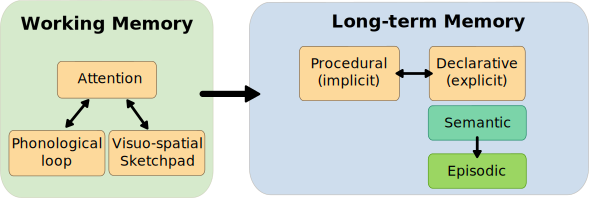
\includegraphics[width=0.9\columnwidth]{memory_models.pdf}
    \caption{Overview of the main types of memories}
    \label{fig|memory_models}
\end{figure}

Most knowledge representation systems offers some kind of memory as a pool of
facts that are not forgotten by the robot until it is halted (this memory is
often refered as a \emph{working memory}, but with a meaning unrelated to
Baddeley's definition). Some systems may propose persistent storages that allow
the robot knowledge to grow over time, while other may offer a larger range of
memory categories, like short term memory (that lasts for a couple of seconds)
or episodic memory (that allows the robot to selectively remember facts
associated to specific events).


%%%%%%%%%%
\subsection{Reasoning Techniques}
\label{sect|reasoning}

\subsubsection{Standard reasoning techniques}

Being based on logical languages to represent the knowledge, most of the
systems we survey allow various forms of \emph{reasoning}.

We call \emph{standard reasoning techniques} techniques based on logical
inference, using resolution algorithms like \emph{forward chaining},
\emph{backward chaining} or \emph{semantic tableaux}.

Main reasoning problems include \emph{concept satisfiability},
\emph{consistency checking} and \emph{instance checking}.

Concept satisfiability verifies if it is possible to find a non-empty
\emph{interpretation} of a concept (or an expression defining a concept) in the
knowledge model. For instance, the formula \concept{Plant} $\land$
\concept{isRed}, which defines the concept of red plants, is satisfiable in a
model \concept{KB} iff $\exists a, $ \concept{Plant}$(a) \land$
\concept{isRed}$(a)$, \ie if we can find at least one red plant $a$ in our
model.

Checking the consistency of a model is equivalent to checking the
satisfiability of each of the concept defined in the knowledge model.

Instance checking consists in verifying that an individual $a$ is an
interpretation of a concept (or concept expression) $C$ in the knowledge model.
A typical example would be that we are provided with an instance
\concept{object1} and we want to know if this object is a kind of
\concept{Bottle} or \concept{Glass}.

Reasoners can then provide other type of inferences, like:

\begin{itemize}
    \item class subsumption (similar to inheritance)

    \item reasoning on roles properties, including:
        \begin{itemize}
        \item entailments based on roles domain and range (for instance, if the
        domain of the role \concept{thinksOf} is known to be
        \concept{ThinkingAgent}, then \concept{thinksOf}$(a, b) \to
        $\concept{ThinkingAgent}$(a)$),

        \item universal, existantial and cardinality constraints (including \concept{allValue}, 
        \concept{someValue}, \concept{hasValue}),

        \item property characteristics (symmetry, transitivity, etc.)

        \end{itemize}

    \item complex concept expressions like: \par \footnotesize \concept{Bottle}
    $\equiv$ \concept{Artifact} {\bf that} (\concept{hasShape} {\bf value}
    \concept{cylinderShape})\footnote{This example uses the \emph{Manchester
    syntax}, \url{http://www.w3.org/TR/owl2-manchester-syntax/}} \normalsize

    \item set operations like: \par \footnotesize \concept{Color} $\equiv$ {\bf
    unionOf}(\concept{blue}, \concept{green}, \concept{orange},
    \concept{black}...) \normalsize

\end{itemize}

\paragraph{Rule Languages}

As mentionned earlier, knowledge models based on description logics can be extended through rule languages.

Intersection of properties is an example of expression that can only be represented with rules: for instance, 

generic SWRL ({\em Semantic Web Rule Language}) rules like: \par
        \footnotesize \concept{looksAt(?agt, ?obj)} $\land$
        \concept{pointsAt(?agt,?obj)} \par $\Rightarrow$ \concept{focusesOn(?agt, ?obj)}
        \normalsize 


\subsubsection{Alteration of the knowledge structure}

In systems

All systems allow to modify the ABox, not always possible to alter the TBox


\subsubsection{Lazy evaluation}
\label{sect|lazy-evaluation}


\subsubsection{Reasoning with uncertainty}


\subsubsection{(Non) Monotonic Reasoning}

\emph{Monotonic reasoning} means that addition of new assertions to a knowledge base
can only extend the set of assertions that can be inferred, while a
\emph{non-monotonic} reasoning scheme may lead to retraction of facts.
McCarthy coined a famous example to illustrate the need of non-monotonic reasoning:

\begin{quotation}
Consider putting an axiom in a common sense database asserting that birds can
fly. Clearly the axiom must be qualified in some way since penguins, dead birds
and birds whose feet are encased in concrete can't fly. A careful construction
of the axiom might succeed in including the exceptions of penguins and dead
birds, but clearly we can think up as many additional exceptions like birds
with their feet encased in concrete as we like. Formalized non-monotonic
reasoning provides a way of saying that a bird can fly unless there
is an abnormal circumstance and reasoning that only the abnormal circumstances
whose existence follows from the facts being taken into account will be
considered.
\end{quotation}

Another important application of non-monotonic reasoning is representation of
change: for example, to make an omelette, you need to crack eggs and wipe them.
The eggs disappear and are replaced by an omelette:

\concept{Egg}$(a) \wedge $ \concept{Egg} $(b) \wedge $
\concept{MakeOmelette}$(a, b, c) \to \lnot $ \concept{Egg}$(a) \wedge \lnot $
\concept{Egg}$(b) \wedge $ \concept{Omelette}$(c)$

The insertion of the proposition \concept{MakeOmelette}$(a, b, c)$ leads to
retraction of other facts. This rule requires non-monotonic reasoning to be
applied.

\emph{Default logic} is one of the formal logic that account for representing
general truth and exceptions to it (for instance, \emph{tomatoes are red, in
general}). However, due to computational complexity of these model (most of
inferences in default logic are known to be $NP$-complete problem), classical
logics and most of the existing reasoners do not allow non-monotonic reasoning.
For instance, the SWRL rule language, usually associated to the OWL-DL ontology
language, do not allow non-monotonic reasoning.

\fxfatal{Make clear 'who does not allow non-monotonic-reasoning': logics? rule
languages? reasoner?}

One important exception if the \emph{Negation as failure} inference rule, as
implemented by {\sc Prolog} for instance, that allows for non-monotonicity, but
only \emph{within the closed world assumption}.

\fxfatal{Give here an example of non-monotonic reasoning with Prolog}

A monotonic system does not theoretically allow for knowledge retractation,
which is an important issue in the robotic context where the world model is
likely to be often altered.  However it is a practical issue only if the
reasoning process is \emph{continuous} during the whole robot's activity
lifespan. It is often possible to stop the reasoner, alter the knowledge, and
restart the inference process on a new domain.
\fxfatal{Rephrase to emphasize that when new evidences appear, it is anyway often a
good idea to restart the reasoner.}

\fxfatal{Mention that the 'change of world' issue can also be dealt with appropriate
time representation.}
\fxfatal{Mention that probabilistic reasoning lead to implicit non-monotonic reasoning}


\subsubsection{Presupposition Accommodation}
\label{sect|presupposition-accomodation}

\emph{Presupposition accommodation} is the ability for the system to
automatically create a context allowing to make sense of a proposition.

For instance, we can imagine a human telling a robot \emph{Please get me the
bottle that is behind you}. If the robot has not yet see what is behind it, it
needs to assume (and represents in its knowledge model) that a undefined bottle
can be found somewhere in the half of space behind it.

A knowledge representation system able to copte with presupposition
accommodation would be able to take into account this (usually under-defined)
information that is not grounded into perception for later inferences.

This ability to imagine a physically state of the world that is not actually
perceived can be seen as the converse of the grounding ability.

Note also that presupposition accommodation implies a bidirectional link of the
symbolic knowledge model with a geometric (or physical) model of the
environment. This article focuses on symbolic knowledge representation systems,
but we shall mention when a KRS explicitly provides support for presupposition
accommodation.

\subsubsection{Prediction, projection and diagnosis tasks}
\label{sect|prediction-projection}

Levesque~\cite{Levesque2008} distinguish two main tasks, the \emph{projection
task} and the \emph{legality task}.

\paragraph{Projection task}: determining whether or not some condition while
hold after a sequence of actions.

\paragraph{Legality task}: determining whether a sequence of action can be
performed starting in some initial state.

\paragraph{Diagnosis}: this corresponds to the ability to rewind on past events
in case of failure to provide possible explanation. This can be seen as the
temporal reverse of the projection task.

\subsubsection{Physics-based reasoning}
\label{sect|physics}

As embodied entities, robots have to interact with physical entities.
\emph{Naive physics reasoning} covers all the everyday reasoning the humans
unconsciouly perform, like taking into account gravity (``if I drop a ball, it
falls down'') or common physical properties of objects (``a glass may break if
dropped'', etc.). Many of the interactions with our everyday environments are
ruled by such laws that are difficult to exhaustively encode.

Some systems \cite{Kunze2011a} rely on external dedicated physics engine to
compute symbolic facts from on-demand physics simulation. This, however,
requires a tight integration between the symbolic model and a geometric model
that carries the geometries and physical properties of objects.

\subsubsection{Planning}
\label{sect|planning}

Making decision based on prediction

\subsubsection{Learning}
\label{sect|learning}

%%%%%%%%%%%%%%%%%
\subsection{Acquiring Knowledge}

\subsubsection{Knowledge acquisition and modalities merging}
\label{sect|knowledge-acquisition}

In the survey inclusion criteria, we have insisted on only considering robotic
systems that acquire knowledge by themselves, during their runtime.

\emph{Acquiring knowledge} means in our context building new statements
(usually as new logical facts) connected to our existing knowledge from
external sources of information. We consider mainly three of them:
proprioceptive/exteroceptive sensors, interaction with other agents, humans or
robots, and remote databases. This process has generally at least two steps:
the information acquisition by itself, and the \emph{transformation} of the
information into knowledge, \emph{aligned} with the robot existing model
(following our terminology for information and knowledge, as discussed in the
introduction).

Knowledge acquision is generally not done directly in the knowledge
representation system. On the contrary, several, if not numerous, external
components are usually required to convert percepts into symbolic facts and to
ground them.

While we do not review in this article all these systems, the whole process of
knowledge acquisition is central in cognitive robotic architecture and the
design of knowledge representation systems can influence or be influenced by
the approach to knowledge acquisition.

In particular, complex robotic systems often require multi-modal perception
capabilities (for instance, a robot can only interpret an utterance like ``this
is a plate'' if it is able to understand gestures, understand natural language
and merge them in a timely manner). Multi-modal interpretation can take place
at various levels, but in many cases (especially if the modalities are of very
different natures, like in the example above) merging will require
symbolic-level reasoning. The KRS has a direct impact on the feasability and
ease of such operations.

\paragraph{Perception}
\paragraph{Interaction}
\paragraph{External sources (Web, upper ontologies, ...)}
\paragraph{Learning}

\subsubsection{Grounding/anchoring strategies}
\label{sect|grounding}

\subsubsection{Ability to automatically create new object instances}
\label{sect|new-instances}

%%%%%%%%%%%%%%%%%
\subsection{Practical Integration in Robotic Architectures}
\label{sect|integration-robot}

\subsubsection{Integration with sensori-motor layers}
\label{sect|integration-sensorimotor}

Ability to ``listen'' to the robot internal structures.

\subsubsection{Integration with executive layers}
\label{sect|integration-executive-layers}

\paragraph{Language integration}

\paragraph{Events}

\subsubsection{Monitoring and debugging}
\label{sect|debugging}

\subsubsection{Is it fast enough? Scalability and responsiveness}
\label{sect|scalability}

%%%%%%%%%%%%%%%%%%%%%%%%%%
\subsection{Knowledge instanciation}

How much knowledge is available? Which content? How big is the knowledge base?

\begin{itemize}
	\item  Which underlying knowledge (\emph{common-sense}, \emph{upper knowledge}\ldots{})
	\begin{itemize}
		\item  top-down approach?
	\end{itemize}

\end{itemize}



%%%%%%%%%%%%%%%%%%%%%%%%%%%%%%%%%%%%%%%%%%%%%%%%%%%%%%%%%%%%%%%%%%%%%%%%%%%%%%%%%%%%%%%%%%%
\section{Surveyed systems}
\label{sect|surveyed-systems}

Table \ref{table|surveyed-systems} presents the fifteen knowledge representation systems surveyed
in this article.

This section briefly presents each of them.

\begin{landscape}
\begin{table}
\begin{center}
\rowcolors{2}{lightgray}{codegray}

%\begin{tabularx}{\textheight}{p{2cm}p{4cm}p{3cm}p{4cm}p{2.3cm}p{2cm}p{2cm}}
\begin{tabular}{p{2.2cm}p{1.6cm}p{4cm}lp{2.4cm}p{3.4cm}p{2.8cm}p{1.5cm}}
\hiderowcolors
{\bf Project} & {\bf Category} & {\bf Authors (Institution)} & {\bf Project homepage} & {\bf Programming language} & {\bf Knowledge model/Logical Formalism} & {\bf Reasoner} & Main reference \\
\hline
\showrowcolors
{\sc KnowRob} & KRS & Tenorth, Beetz \par (TU Munich) & \url{http://ias.in.tum.de/kb/wiki} & {\sc Prolog} & {\sc Prolog} + OWL-DL & Custom \par ({\sc Prolog}) & \cite{Tenorth2009a} \\
ORO & KRS & Lemaignan, Alami \par (LAAS-CNRS) & \url{oro.openrobots.org} & {\sc Java} & OWL-DL ({\sc Jena}) & {\sc Pellet} & \cite{Lemaignan2010} \\
PEIS KR\&R & KRS & Daoutis, Coradeshi, Loutfi, Saffiotti \par (Örebro Univ.) & \url{www.aass.oru.se/~peis} & {\sc C}, {\sc CycL} & CycL (1st and 2nd order logics, modal logics) & & \cite{Daoutis2009} \\
CAST Proxies & Ubiquitous & Wyatt, Hawes, Jacobsson, Kruijff (Brimingham Univ., DFKI Saarbrücken) & & & Amodal proxies & & \cite{Jacobsson2008} \\
Golog & Language & Levesque (Toronto Univ.) & & {\sc Prolog} & & & \\
NKRL & Language & Zarri et al. \par (Paris Est Créteil Univ.) & & NKRL & & & \cite{Sabri2011} \\
GSM & & Mavridis, Roy \par (MIT MediaLab) & & & & & \cite{Mavridis2006} \\
OMRKF & & Suh et al. \par (Hanyang Univ.) & \url{incorl.hanyang.ac.kr/xe/?mid=symbolic_reasoning} & ? & Horn Clauses & ? & \cite{Suh2007} \\
DY-KNOW & & Heintz, Dowerty \par (Linköping Univ.) & & & & & \cite{Heintz2004} \\
Ke Jia & & Chen et al. \par (Univ. of Science and Technology of China) & & & & & \cite{Chen2010} \\
 & & Varadarajan, Vincze \par (TU Wien) & & & & & \cite{Varadarajan2011} \\
 & & Kaelbling, Lozano-Pérez \par (MIT CSAIL) & & & & & \cite{Kaelbling2011} \\
ARMAR & & Schmidt-Rohr (Karlsruhe TH) \\
 & & Hertzberg (Osnabrück Univ.) \\
 & & (DFKI Bremen) \\
 (based on {\sc KnowRob} & & (JSK) \\

\hline

%\end{tabularx}
\end{tabular}
\end{center}
\caption{List of surveyed systems. Projects are listed by category (\emph{KRS} for systems that are explicit knowledge representation and reasoning modules, \emph{Ubiquitous} for systems where knowledge processing is fully distributed, \emph{Language} for languages used as KRS on robots), then names.}
\label{table|surveyed-systems}
\end{table}
\end{landscape}

\fxfatal{Bielefeld -> could not find much...}
\fxfatal{Kollar/Tellex -> really focusing on the natural language grounding}

\subsection{KnowRob}
\label{sect|knowrob}

\subsection{ORO}
\label{sect|oro}

\subsection{PEIS KR\&R}
\label{sect|peis-ecology}


{\sc PEIS Ecology}~\cite{Saffiotti2005} is a software \emph{ecosystem} that aim to binds autonomous
robotics with ambient intelligence (network of sensors). \emph{PEIS} stands for
\emph{Physically Embedded Intelligent System}: every robots or intelligent
device in the environment is abstracted as a PEIS.

Each PEIS physical component is running a \emph{PEIS Kernel} instance. Communication
between instance relies on a custom P2P communication protocol.

The PEIS architecture allows for adding new abilities through software components sharing the common \emph{tuple space}.

We survey here the semantic layer~\cite{Daoutis2009}, referred as \emph{PEIS KR\&R}, that includes symbolic representation and reasoning.

% More in details:
% - object identification based on viewpoint independent SIFT features
% - formalized anchoring system that explicitely match percieved attributes to predicates
% - Cyc predicates
% - ground 12 colors, based on a paper on color perception. Could be useful for us.
% - idem, they cite a paper on what spatial relations to compute
% - location of objects based on a previously provided semantic map (but not much on this semantic map)
% - two "memories": the robot memory stores the current list of percieved objects ; the archive memory stores what is not percieved anymore
% - uses directly Cyc (ie, 250 000 common sense concepts...), via CycL language -> 2nd and higher order logics (quantification over predicates, functions, etc)
% Remark: using 2nd order logic (ie meta statements), it would be easy to store the knowledge of each agent
% - disambiguation in concept name by asking human to decide amongst all concepts known by Cyc
% - template based natural language
% - experiment conducted in a "smart" indoor environmement + simple robot

\paragraph{Knowledge model} The PEIS Knowledge representation system relies on
the {\sc ResearchCyc} and {\sc CycL} language to represent knowledge. The {\sc CycL} language
allows to represent first order logic sentences and has extensions for modal logics and higher order logics.

\fxfatal{Is modal logics and higher order logics actually used in PEIS?} 

As a system relying on {\sc CycL}, contexts can be expressed as
\emph{microtheories}: the truth or falsity of a set of statement depends of the
\emph{microtheory} in which these statements are evaluated.

\fxfatal{OWA/CWA?}

\begin{figure}
	\centering
	\includegraphics[width=0.9\columnwidth]{peis-architecture.pdf}
	\caption{The PEIS knowledge representation system, taken from~\cite{Daoutis2009}}
	\label{fig|peis-archi}
\end{figure}

The PEIS KR\&R system is deeply integrated to the general PEIS Ecology
\emph{smart} environment. Figure~\ref{fig|peis-archi} gives an overview of the
interactions between PEIS knowledge processing layers.

\paragraph{Knowledge Acquisition} The primary source for knowledge acquisition
is perception.  The PEIS ecosystem provides a SIFT-based object recognizer used
in conjunction with ceiling cameras for object localization.  Other perceptual
modalities are available (like human tracking, ambient environment monitoring).

A template-based natural language parsing system may also be used to add new
assertions to the system.

The system can ask the human for help to disambiguate between concept names.

\paragraph{Anchoring} Daoutis et al. formalize the issue of anchoring as
finding a \emph{predicate grounding relation} $g \subseteq \mathcal{P} \times
\Phi \times D(\Phi)$, where $\mathcal{P}$ is a set of predicate symbols, $\Phi$
a set of percept's attributes, and $D(\Phi)$ the domain of these attributes.

In the current implementation, object category (returned by the SIFT
classifier), color, location, spatial relations (both topological -- \emph{at},
\emph{near} -- and relative to the robot -- \emph{left}, \emph{behind}, etc.)
and visibility are the five classes of extracted attributes.

\paragraph{Integration in the robot architecture}
\label{sect|peis-integration}

The PEIS framework offers through the \emph{PEIS middleware} a practical way to
insert a new component into the shared \emph{tuple space}.  Thus, the KR\&R
module can be seemlessly integrated into the PEIS ecosystem.

\subsubsection{Notable experiments}
\label{sect|peis-expe}

\subsection{NKRL}
\label{sect|nkrl}

\emph{NKRL} stands for \emph{Narrative Knowledge Representation Language}.
While this language is developped since a long time by Zarri~\cite{Zarri1997,
Zarri2008}, recent research direction include application to the robotic
field~\cite{Sabri2011}. NKRL is not {\it per-se} a knowledge representation
system, as it is primarily a language. However, it is used as the
representation and reasoning mechanism for robots by Sabri et al.

\subsubsection{Intrinsic language features}
\label{sect|nkrl-intrinsic-features}

\paragraph{Expressiveness}

\subsubsection{Integration with physical world and in the robot architecture}
\label{sect|nkrl-integration}

...seem to be mostly WIP...


\subsection{CAST Knowledge model}
\label{sect|cast}

CAS (\emph{CoSy Architecture Schema}) Toolkit~\cite{Hawes2007} is a
comprehensive toolkit aimed at builduing cognitive architectures for robots
through a set of interconnected SAs (\emph{subarchitectures}). The CAS does not
expose a central knowledge base as seen in previous works. It instead
represents knowledge as unrooted \emph{proxies}. Thoses proxies are formally
defined in \cite{Jacobsson2008} as $p= \langle F_p, u_p \rangle$ where $F_p$ is
a set of instanciated features (like $\phi^{Colour}_{red}$) and $u_p$ a
\emph{proxies union} that form an equivalence class corresponding to one
entity.

A union of proxies forms a global amodal representation of an entity, that can
be explicitely shared and manipulated. Being not centralized, the knowledge
model can be qualified of \emph{ubiquitous}. Futhermore, knowledge source in
the CAS architecture is tightly bound to the on-line grounding process (be it
grounded in perception or in dialogue). While nothing seems to prevent it, no
{\it a priori} knowledge (including common-sense knowledge) is used.

Knowledge sharing is ensured by the event mechanism of CAST: modules can
monitor proxies for alteration by other modules. Jacobsson et al. mention how
this can apply to reinforcement learning: the vision module creates a proxy for
an orange object. This proxy get monitored by a learning module. In parallel,
the proxy is bound to an union by the natural language understanding module
that add new a feature like \emph{"this object is a fruit"}. The learning
module is called back, and can add this new information to its model.

In the presented implementation, the CAST knowledge model does no allow for
effectively representing actions or temporal information.\fxfatal{What about reasoning? can they retrieve for example 'all proxies for colorful objects'?}

\subsection{OMRKF}
\label{sect|omrkf}

The Ontology-based Multi-layered Robot Knowledge Framework~\cite{Suh2007}
(OMKRF) is a knowledge representation system based on four inter-related
\emph{classes} of knowledge (Figure~\ref{fig|omrkf}). It proposes a layered
approach to knowledge representation that allows to integrate the grounding
process to the knowledge representation process. OMRKF knowledge model is
implemented with Horn clauses.

\begin{figure}
    \centering
    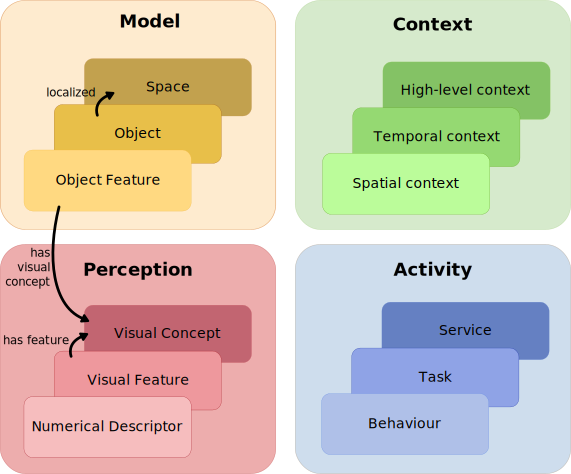
\includegraphics[width=0.8\columnwidth]{omrkf.pdf}

    \caption{OMRKF organizes knowledge into four \emph{classes}, each composed
    of three \emph{levels}. The figure shows some examples of link between
    knowledge classes and knowledge levels. Based on~\ref{Suh2007}.}

    \label{fig|omrkf}
\end{figure}

Each level of knowledge is build as three stages of ontological realization: a
\emph{meta-concept} (the level itself, like ``temporal context'', ``behaviour''
or ``object feature'', a taxonomy of concepts inside this level (for instance
$cup : Object \sqsubseteq tableware : Object$) and an instanciation of the
taxonomy ($cup1 : cup$).

Environment is represented in OMRKF in the $space : Model$ knowledge level as a
classical three layers mapping (metric, topological and semantic maps). Objects
(in $object : Model$) are localized in $space : Model$ through Voronoi nodes.

The knowledge class $Context$ proposes an explicit statement of spatial context
(mostly geometric relations between objects), temporal context and a more
general \emph{high-level} context, inferred from spatial and temporal contexts.

Finally, the $Activity$ knowledge class store coumpound actions in a HTN-like
structure, exploited at run-time by a planner.

\paragraph{Experiments} Experiments conducted with OMRKF include finding
kitchen objects and reporting about their state to a human.  This experiment
also shows how OMRKF can deal with objects only partially matched by their
descriptor by introducing a $candidate()$ function.

%%%%%%%%%% Underlying knowledge model table %%%%%%%%
\begin{table}
\begin{center}
\rowcolors{2}{lightgray}{codegray}

\begin{tabular}{lp{4cm}}
\hiderowcolors
{\bf Project} & {\bf Common-sense \par knowledge source} \\
\hline
\showrowcolors
{\sc KnowRob} & {\sc OpenCyc}, processed web content, custom OWL-DL ontology \\
ORO & {\sc OpenCyc}, custom OWL-DL ontology \\
PEIS Ecology & {\sc ResearchCyc} \\
DY-KNOW & \\
OMRKF & {\it A priori} knowledge structure and axioms, custom set of instances\\
GSM &  \\
NKLR &  None \\
CAST Proxies &  None \\
Wrighteagle & \\
Vincze & \\
ARMAR &  \\
Hertzberg (Osnabrück) & \\
(DFKI Bremen) & \\
(JSK) & \\

\hline

\end{tabular}
\end{center}
\caption{Underlying knowledge sources for each project}
\label{table|knowledge-sources}
\end{table}


%%%%%%%%%%%%%%%%%%%%%%%%%%%%%%%%%%%%%%%%%%%%%%%%%%%%%%%%%%%%%%%%%%%%%%%%%%%%%%%%%%%%%%%%%%%
\section{Summary of Approaches}
\label{sect|summary}

\begin{landscape}
\begin{table}
\begin{center}

\begin{tabular}{cp{4.5cm}ccccccccc}
\toprule
\multicolumn{2}{c}{\bf Category} & {\sc KnowRob} & {ORO} & {\sc PEIS} & {\sc CAST} & {\sc Golog} & {\sc NKRL} & {\sc GSM} & {\sc OMRKF} & {\sc DY-KNOW} \\

\midrule

\multirow{5}{0.7cm}[-0.2cm]{\turn[1.5cm]{90}{\bf Expressive power}} & Logical formalism & Prolog & OWL-DL & {\sc CycL} &  &  &  & & Horn clauses & \\
 & Expressive power & & & & & & & & &  \\
 & OWA/CWA & CWA & OWA & & & & & & & \\
 & Modeling uncertainty & +++ (extension) & & & & & & & + (\emph{candidate} entities) & \\
 & Meta-cognition & ++ & ++ & & & & & & & \\
\hline
\multirow{6}{0.2cm}{\turn{90}{\bf Model}} & Representation of space & & & & & & & & ++ &  \\
 & Representation of temporality & & & & & & & & + &  \\
 & Context & & & & & & & & ++ &  \\
 & Alternative worlds & & +++ & & & & & & &  \\
 & Introspection & + (SRDF) & & & & & & & &  \\
 & Memory & & + & & & & & & &  \\
\hline
\multirow{10}{0.2cm}{\turn{90}{\bf Reasoning}} & Standard FOL reasoning & +++ & +++ & & & & & & &  \\
 & Knowledge structure alteration & & ++ & & & & & & &  \\
 & Lazy evaluation & +++ & & & & & & & &  \\
 & Reasoning under uncertainty & ++ (extension) & & & & & & & & \\
 & Non-monotonic reasoning & & & & & & & & &  \\
 & Presupposition accomodation & & & & & & & +++ & &  \\
 & Prediction, projection, diagnosis & & & & & & & & &  \\
 & Physics-based reasoning & +++ (extension) & & & & & & & &  \\
 & Planning & + & +++ (external module) & & & & & & &  \\
 & Learning & & & & & & & & &  \\
\hline
\multirow{3}{0.7cm}{\turn[1cm]{90}{\bf Knw. acq.}} & Acquisition techniques & & & & & & & & &  \\
 & Grounding & & & & & & & & &  \\
 & Instanciation & & & & & & & & &  \\
\hline
\multirow{4}{0.2cm}{\turn{90}{\bf Integ.}} & ...with sensori-motor layers & & & & & & & & &  \\
 & ...with executive layers & & & & & & & & &  \\
 & Monitoring and debugging & & & & & & & & &  \\
 & Performances & & & & & & & & &  \\

\bottomrule

%\end{tabularx}
\end{tabular}
\end{center}
\caption{Main domain of contribution of each surveyed systems. Rating goes from +++ (major focus) to + (secondary interest). An empty cell means that 
the system does not consider this domain.}
\label{table|contribution-by-systems}
\end{table}
\end{landscape}


This section tries to summary the various approaches we surveyed in the
previous section.  This summary does not exactly follow the list of compared
features presented in section~\ref{sect|features}. We have organized
it along four axis: \emph{what can be represented?}, \emph{How knowledge is
created and grounded?}, \emph{What can be done with the knowledge?} and
\emph{How to use knowledge in the whole, larger robot architecture?}.

\subsection{Expressiveness: what can we represent in the current state-of-the-art?}
\label{sect|summary-expressiveness}

\begin{itemize}
	\item expressiveness
\end{itemize}


\subsection{Creating and grounding knowledge in the physical world}
\label{sect|summary-grounding}

\fxnote{Mention symmetry and research of invariants \cite{Henderson2011} as a process to create knowledge?}

\begin{itemize}
	\item which knowledge modalities can be merged
	\item which grounding strategies
\end{itemize}


\subsection{Exploiting knowledge}
\label{sect|summary-knowledge-sources-reasoning}

\begin{itemize}
	\item which common-sense knowledge is used
	\item what kind of reasoning is made
	\item introspection
\end{itemize}


\subsection{Using a knowledge representation system in a larger robotic cognitive architecture}
\label{sect|summary-integration}

\begin{itemize}
	\item a priori evaluation/lazy evaluation and trade-offs (relations to events, scalability, detection of inconsistencies,...)
	\item relation with planning (action representation, temporal representation...)
	\item API/bindings/integration into executive layers
\end{itemize}

%%%%%%%%%%%%%%%%%%%%%%%%%%%%%%%%%%%%%%%%%%%%%%%%%%%%%%%%%%%%%%%%%%%%%%%%%%%%%%%%%%%%%%%%%%%
\section{Towards the next generation of Knowledge Representation Systems for Robotics}
\label{sect|conclusion}

\subsection{Current shotcomings: what is not successfully covered by current systems}

\subsection{Towards a new design}

%%%%%%%%%%%%%%%%%%%%%%%%%%%%%%%%%%%%%%%%%%%%%%%%%%%%%%%%%%%%%%%%%%%%%%%%%% 
\section*{Acknowledgements} 

%%%%%%%%%%%%%%%%%%%%%%%%%%%%%%%%%%%%%%%%%%%%%%%%%%%%%%%%%%%%%%%%%%%%%%%%%% 

\bibliographystyle{ieeetr}
\bibliography{biblio}


\end{document}
